% ============================================================
% PHẦN Faster-GS bổ sung — Slide: MCMC densification (thay thế, không bật mặc định)
% ============================================================

% --- Slide (Faster-GS 5/8) ---
\begin{frame}{MCMC densification — có sẵn nhưng KHÔNG bật mặc định}
\footnotesize
\begin{itemize}
    \item Đây là phương án thay thế (\textbf{3DGS-MCMC}) cho densify chính của FastGS, đã cài đặt đầy đủ, đúng toán trong code -- nhưng \textbf{không} được gọi trong control-flow mặc định.
    \item Lý do: \alert{xung đột kiến trúc thật} -- MCMC và \texttt{densify\_and\_prune\_fastgs} loại trừ lẫn nhau, không thể chạy cùng lúc trên cùng tập Gaussian.
\end{itemize}
\vspace{0.3em}
\textbf{Closed-form relocation (3DGS-MCMC, Eq.\,9):} khi 1 Gaussian chết được thay bằng resample + nhân bản $n$ bản sao,
\[
\alpha' = 1-(1-\alpha)^{1/n}
\]
opacity mới mỗi bản sao, đảm bảo tổng hiệu ứng alpha-blending không đổi (khi $n=1$ thì $\alpha'=\alpha$).

\textbf{Noise injection:}
\[
\Delta xyz = lr\cdot\sigma(0.5-100\alpha)\cdot\Sigma\cdot\varepsilon
\]
Gaussian opacity thấp di chuyển nhiều hơn (khám phá), opacity cao gần như đứng yên.
\begin{itemize}
    \item[$\Rightarrow$] \texttt{densify\_and\_prune\_fastgs} (đóng góp chính của FastGS) vẫn là cơ chế densify duy nhất luôn bật; MCMC giữ nguyên trong code, sẵn sàng bật thủ công nếu muốn benchmark sau.
\end{itemize}
\centering
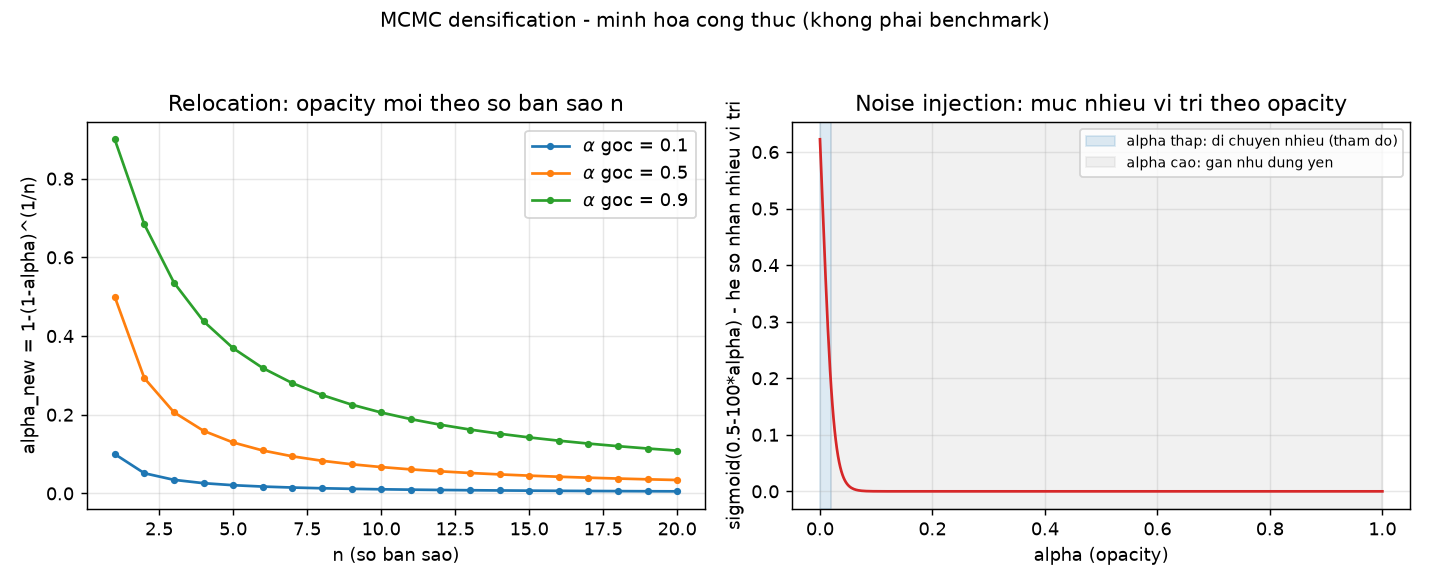
\includegraphics[width=0.38\linewidth]{../BOOK/adc_figures/12_mcmc_relocation_formula.png}
\captionof{figure}{\footnotesize $\alpha'$ theo $n$ và hệ số nhiễu sigmoid theo $\alpha$ (công thức toán, không phải benchmark)}
\end{frame}
